\documentclass{article}

\usepackage{hyperref}
\usepackage{graphicx}

\begin{document}
\title{Tarot: An Informal Self-Experiment}
\author{Matthew Scott}
\maketitle

\section{Introduction}
Tarot is a game of correspondences.  Rather than aiming to strictly
'divine' the future, we look for correspondences between the cards laid
out before us and the rest of our lives - how this card relates to our
past, what this card means in the present, and using that card to divine
a new path through life.  Tarot can change the way we act, can help us
search the depths of our subconscious and memories to help explain the
events of the past, and will show us new ways to work with the future,
ways that we would never have thought of before without some outside
influence, doing so all while being impersonal, keeping our deepest
secrets, and never telling a soul about these correspondences.

I got interested in Tarot through various sources.  In my exploratory
high school years, I had a few friends and a few relationships with some
brilliant people with diverse interests, and a few of them showed me
different aspects of tarot at different points in my career.  Despite
having two very scientific and skeptical parents, I developed something
of an interest in occult systems such as Tarot and wound up frequenting
a bookstore catering to those interests in my home town.  

At one point, while purchasing my first deck of my own, I was offered a
free reading with my own deck of cards from an established cartomancer
at the bookstore.  The reading proved to be one of the most powerful
experiences in my life up to that point.  From then on my interest grew
further, leading to many more purchases of decks and books, as well as
further research online and in libraries in Tarot as well as other
occult systems.  To this day, many of my readings still follow the same
general plan as that original one so many years ago.

I have not forgotten my heritage, though, and the respect for the more
commonly accepted sciences ingrained in me by my parents.  I thus
decided to embark on a bit of an informal self-experiment, following the
guidelines of the scientific method to test how working with the Tarot
as a tool to explore deeper within myself might change the way I
perceive the world around me, alter the way I act by forcing me to think
through situations in a different way.  This experiment also acts as a
bit of a slice-of-life diary, with each reading providing a view of
what's going on in my life at the time - the issues that are concerning
me, and all the hopes and fears that have built up to that point.

%%%%%
\section{An Informal Self-Experiment}

%%%%%
\subsection{Questions}
\begin{itemize}
	\item How does tarot work?
	\item How does learning to work with the tarot affect a person?
	\item Does mindfully working with the tarot generally lead to a different method of dealing with events in the past?
	\item Does mindfully working with the tarot generally lead to a different consideration of the future?
	\item How does working with the tarot affect the way a person deals with events and their position in time?
	\item How does the conscious application of a defined set of archetypes change the way a person deals with a situation?
	\item How does the person respond to such questions as these above being applied to them?
\end{itemize}

What I aim to learn from this experiment is basically what would happen
by changing a part of my life.  I don't want to see into the future,
necessarily.  Rather, I would like to become more cognizant of the
present, to take the past into account, and to integrate all levels of
myself into my day-to-day life: conscious, subconscious, and
unconscious.  While the questions listed above are the specific ones,
the more general overview would be this: if I were to consciously try to
change my outlook on life through the use of this tool, what would
happen?  What would change about me as a person, not just the path my
life was taking?

%%%%%
\subsection{Observation}
\begin{quote}
We come to the notion that the Tarot works precisely because it makes no
sense.  The information exists.  Our unconscious selves already know it.
What we need is a device to act as a bridge to conscious perception.
\cite{pollack97}
\end{quote}

The modern Tarot deck is made up of 78 cards - there are 56 minor arcana
and 22 major arcana cards.  All of these cards represent different
archetypes, or general ideas about different aspects of life, humanity,
and the self.  More than simply divining the future, one my seek out
correspondences between situations at hand, in the past, or possibly in
the future through these archetypal images, laid out within the
framework of the cards and how they relate to each other.  One can
utilize a 'spread', a pattern in which to lay the cards with each of
their positions holding a predetermined meaning so as to deepen the
meanings of each card.  Just as frequently, however, one may let the
cards, the reader, or the querent determine the positions of those
cards, divining meanings for them as the reading progresses.

There are many different views on Tarot.  By far, the overwhelming
majority of people in todays world put little or no stock in divination
of any sort, and would just as soon leave any introspection in the hands
of those with 'Ph.D' tacked on the ends of their names.  Of those whose
opinions do not favor Tarot, there are further divisions: some may have
humored a cartomancer and had a reading done for themselves and disliked
it for one reason or another, having been scared by it; some may have
difficulty thinking of those who deal in such things as actively harmful
frauds; and everything in between.  On the other side, of course, there
are those who see the cards as a window into the future, those who use
them strictly for introspection, those who use them for various magical
purposes, and, again, everything in between.

This document is hardly meant to be a dissertation on the cards
themselves, nor the varied opinions on their meanings or acceptance in
the world today.  For further information, please look up the
information in the bibliography, as others can surely tell those stories
far better than I.  My aim is only to explore the way that the cards can
influence life.  When I began college, I saw that those around me
weren't focused on growing or changing, and in fact, many had remained
the same person that their parents had molded them into years back,
simply refusing to change.  Not only did that idea of changing who I am
in however subtle a fashion appeal to me, I felt that allowing this
change instead of stagnation would mean that I was actively working to
make myself a better person and doing my best to better the lives of
those around me.

%%%%%
\subsection{Hypothesis}
I feel optimistic about this experiment.  I have rarely ever taken an
active role in the way my life changes, and I think that by guiding it
in this small way, I can improve the way that I deal with what happens
to me, improving the integration of new information in order to become a
better person as a whole.  I also expect that, by being more easily able
to comprehend the world around me and the people in it in reference to
my own worldview, I will be able to affect those around me in a
possitive manner, in effect, being a better person for them.

%%%%%
\subsection{Procedure}
My goal is to do 78 readings of the Tarot with the goal of at least one
reading per day.  For each reading, I will gather information about the
background of the situation, the layout of the cards and the disposition
of the deck, and finally, an analysis of the cards and the reading,
including the effect that the reading had on me as a person.  These
readings will be mostly for myself in my day-to-day life, but I will
also attempt to read for others as well, recording the way the reading
made me feel and any insights that will be applicable in my own life.

When the 78 readings are completed, I will attempt to analyze the
information from the collected write-ups of the readings, looking for
changes over time in the way I interacted with the world around me and
how I felt as a whole.  These trends will be described in as much depth
as possible in order to explore how the conscious utilization of the
Tarot to change my life truly affected me and, hopefully, those around
me as well.

%%%%%
\section{Experimental Data}
\subsection*{Preliminary Introduction}
As these readings are very personal in nature, I feel the need to
introduce myself before just jumping right into portions of my life,
lest they make no sense at all.

I was born Matthew Joseph Scott in January, 1986 to Donna Karr and Ron
Scott, two engineers with the minds of scientists.  I was raised a
skeptic and an atheist.  Life was uncomplicated: everything that could
be explained, was, and anything that couldn't was set aside as an
unknown until it could be explained with no further thoughts on the
matter.  Of course, when you tell a young child not to do something,
that's a very effective way to invite them to do it in secret if
possible; I was told not to concern myself with the unexplainable
matters of religion, mysticism.  Thus it was that I began acquiring my
secret stash of information on all of those subjects, beginning with a
King James bible given to me by a camp counsellor, working up to a
modest library of books dealing with topics ranging from the ``big five''
religions and reiki to the history and use of drugs.  I have already mentioned a
little about my introductions to Tarot.

That leads to me today, August 13, 2008: I am a student in the music composition program
at Colorado State University in Fort Collins, Colorado.  After trying
(and failing) to be a biochemist, I've accepted that I make a far better
musician and publisher than a scientist, but the need to explain, to
experiment, and to experience the world around me remains.

To lend even more specifics to the situation, I was only recently
accepted into the composition program after spending nearly four years
in music education, finding myself disillusioned with the American
public education system.  This means that my four years of paid tuition
promised by my dad are up, and I must begin paying for my own tuition
from my earnings.  I work at the campus library as technical support,
and I am currently dealing with some problematic homophobia from my boss
and coworkers there.  On top of that, just a few months ago, I underwent
a very difficult breakup with my boyfriend at the time.  I ``rebounded''
onto another friend of mine, but as soon as we started getting close to
each other, he had to move down to Denver, Colorado, an hour's drive
away.  

It was this combination of stressors that lead me to look into
creating my own change in life.  This jumble of emotions and ideas is
what I am right now, and I want see what I can make of that by being
more mindful of my life, guiding it where I can, and becoming a better
person, using the Tarot as a tool.

%included files, one for each reading
\subsection{August 13, 2008}
\subsubsection*{The Background}
I've been feeling pretty pessimistic lately.  Andrew still weighs
heavily on my mind, and I'm finding out slowly just how deeply I had
entrenched him into my life.  I was really pretty torn up when he left
me, and everything was made worse when I found out that he did so simply
to be with someone he was already nearly dating behind my back.  Last
night, however, I found out that they were \emph{moving} in together in New
York, despite all his plans to \emph{move} out with me in Colorado.  Feeling
deeply hurt, I stopped watching his journal, and blocked him from
communicating directly with me.  I had done my best to wish them luck, and
now I feel as if I'm just having my nose rubbed in the ruins of our
relationship, so I'm breaking off all contact.  I'm telling myself that
I need to do this in order to get over him and \emph{move} on with the rest of my
life, but really, I'm sure it's little more than a passive aggressive
way for me to get back at him for telling me he'd keep in touch and then
doing this.

All of this seems rather petty in light of my growing feelings for
James, and the concerns I have with him now.  That he \emph{moved}
away from me shortly after we got together certainly isn't helping
things.  It's not the reasons that he \emph{moved} that bother me, of
course, simply that, after my previous relationships, adding that extra
element of distance makes me very, very nervous for the future of this
one, even if it's only down to denver.  I can hardly \emph{move} down 
to join him until I'm finished with school, too.

Finally, the added financial burden of my own tuition is beginning to
worry me a good deal more.  I seem to be \emph{stuck} in this
ceaseless cycle of sleeping in too late and spending all the money I
make on things I don't really need, whereas I really shouldn't let my
wants \emph{hinder} my needs.  I may want that new rifle, but I need
to finish school!

All this pessimism has served to do little more than \emph{block} my
creativity.  I have written only about 30 measures of real music this
summer, as the weight of my emotions keeps \emph{forcing me to stop}
before I feel like I've accomplished much.

As may be evident, I'm having a real problem with \emph{movement} and
the \emph{inability to move}.  I feel stopped up in many ways, as if
the world --- particularly those close to me --- race on by without me.
And so I laid out the cards\ldots

\subsubsection*{The Drawing}
With my dark mood, I chose Aleister Crowley's
\textbf{Thoth}\cite{tarotThoth} deck to do the
reading, figuring that the bright and attractive colors of the RWS deck
didn't quite match what I was feeling.  I wasn't feeling simply down,
either, or I might've chosen the Aquarian deck for its dreary, clouded
look.  I wanted the sharp, geometric shapes and smart color choices of
Lady Frieda Harris' cards to fill out my mood.

I shuffled and shuffled and shuffled until I finally felt I was ready,
and then went through the process of drawing the cards shown to me so
long ago.  Since my emotions where seemingly holding up my life, looking
for resolution, I let them choose the cards, fanning them between my two
hands until I felt that little tug at my subconscious, saying `draw that
card!'.  My intellect continued to take the back seat as my fingers
arranged the cards, face down, into the pattern that I thought they
would best fit when flipped, and for the most part, they chose well.

The pattern started with a card in the upper left, leftmost of a row of
three cards that moved down and to the right.  Directly above the last
card and in line with the leftmost card was another, and directly to the
right of that was a card with another one overlapping the upper-right
hand corner.

From left to right, the cards were:
\begin{itemize}
  \item 6 of Wands, `Victory'
  \item Queen of Disks
  \item 5 of Wands, `Strife'
  \item Above the previous card, 6 of Swords, `Science'
  \item To the right of the previous card, Princess of Swords
  \item Overlapping the upper-right hand corner of the previous card, 4
  of Wands, `Completion'
\end{itemize}
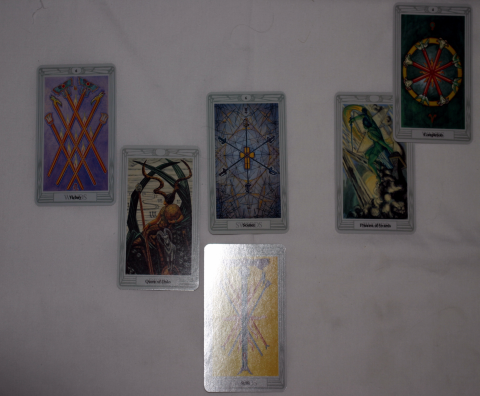
\includegraphics{image8-13-08.png}

\subsection*{The Reading}
The theme of movement became more and more evident as the cards were
flipped over, one by one, starting from the left of the board.  Wands
is the suit of fire, that which is never still.  If nothing else, fire
moves downwards and outwards as it consumes, while air, water, and earth
can all be relatively motionless.  

While the wands start out as a roaring bonfire of problems, the dwindle 
down toward the Ace to the quiet glow of a candle's flame, and the six 
is right when things begin to turn towards calm.  As was mentioned
before, fire moves downwards as it consumes, and, in fact, the first
thing that I noticed about this card was that the small flames in the
vertices of six crossed wands look as if they're forming an arrow
pointing downwards, or else that they're small concerns settling down to
the bottom of the container, relaxing.  This, I feel, is what I may be
going through now.  Despite the problems it caused me, the recent break
up is starting to become less pertinent, I am learning to deal with
James' new distance, and I do see that it is possible for me to pay my
tuition.

Taking this as my cue, I turned over the next card to the right and
slightly lower than the six, revealing the Queen of disks.  Of all of
the cards in the Thoth deck, this one is my favorite.  Many of the minor
arcana cards are little more than pip cards, and most of the court cards
of other suits are dynamic, busy images, whereas the Queen of disks sits
serenely.  Hers is the knowledge of magic of nature, and she sits
ensconced in her angular fronds, looking out over a dry valley with a
snaking river.  This, I think, is the very description of peace in
wisdom.  She is content in life, but not uncomfortable without, a
balance of emotional and intellect that echos through all of the disks.
This card shows me what I've wanted to be ever since I saw it, and I
feel that I'm starting to settle towards it, getting closer to that
ideal.

I turned over the two cards next to it at the same time, as they were in
the same vertical plane.  This revealed two more cards of movement.  The
Golden Dawn (the society of which Crowley was a member, and the source
of inspiration for this deck) label for the lower card is strife, but not
only does the card not give the impression of strife, but the other
common interpretation gives a different impression, as well: that of
striving.  The 5 of wands is a card of battle, but the card of discourse and
games, where there is action, even against another person, but
purposefu and with rules, not unfair, uncivil acts of strife against
another.  Its lower indication indicated to me the subconscious or
unconscious, showing me how my emotions where striving against each
other and against me, but that it was fair, there was a reason, and that
its not strife without rules.

The upper card, the more conscious of the two, is in elemental
opposition to the Queen of disks.  That is, swords and disks, air and
earth, do not mix well, and this alters the meaning of the cards,
bringing out the darker side of both the Queen and this, the 6 of
swords.  It shows that, while the Queen may be comfortable with the idea
of that lifeless desert behind her, she remains forever ensconced in
the life-filled oasis.  To apply the analogy, I may find the idea of
that barren desert of completely settled emotions perfectly acceptable,
but I'm too caught up in my ways, too blinded by intellect,
internalization, and change to let my emotions settle down --- I may
internalize a lot of things, but I'm letting that hinder myself as the
world changes around me.

The Six of swords itself is another card of movement, but rather than
physical movement, this is the movement of an idea or emotion through
time, such as the path that mourning takes.  Something isn't quite right
with the path as it is, though, with the influence of the Queen: the
swords are the suit of silence, and that has me stuck.  Having to take
all of this emotion from the breakup into myself without saying anything
is damaging the way I move through my life, hindering that necessary
passage of mourning while keeping the emotion smoldering.  This shows
the need for communication and action --- the card being above that
subconscious five suggests its more conscious and active role --- in
order to help these issues resolve themselves.

So what about the last two cards?  I turned them over to find the Four
of wands covering the corner of the Princess of swords.  The Princess of
swords, as the earthy side of air, shows the fixation of the volatile,
the ideas made real (she even wears the visage of Medusa on her helmet).
This, to me, was a strong suggestion that I needed to apply my ideas, to
bring them to fruition.  All of the cards before me were giving me a
path and this was saying that, if I followed that path and brought it to
reality, it would be the basis for the card that was above and
overlapping the Princess, the Four of wands, labeled `Completion'. 

More than simply the end of a process, this card shows integration.  The
four wands form a square, their points form an octagon, they are bound
in a circle, everything is integrated.  This is not saying ``Do these
things and everything will magically be resolved,'' this is saying
``Everything was, is, and will be interconnected, forever.''  If I look
to change myself, something else connected to me will change; if I move
forward in my life, I will move forward with a whole host of
opportunities and emotions.  I have always been `complete', whether or
not I have a problem, and I'm certainly realistic enough to realize that
as soon as these problems are resolved, a new set will have cropped up
for me to deal with, but that's okay, they're a \emph{part} of me, and
as soon as I can learn to integrate them into myself (perhaps by doing
what the cards have suggested), it will be easier for me to accept that.

\subsection{August 14, 2008}
\subsubsection*{The Background}
Despite yesterday's fairly positive reading, I'm still operating in that
pessimistic sort of vein.  While less focused on relationships, the
question of money is still bothering me quite a bit, and that's leading
to me being rather down on myself about other things.

In particular, I'm rather concerned about my ability to focus on one
thing for any extended period of time.  The most obvious object of this
focus is this project itself.  I worry that I can't complete even 78
readings for myself and others.  This is a perennial problem for me, and
I often find myself flitting between interests, whether or not I have
completed any projects begun in the previous interestes.  For example,
recently, I've gone through cooking, brewing, my own small business,
programming, guns, and so on.

What's concerning me is that I worked on the problem of being stuck, and
I'm afraid that, once I start moving again, I'll fall into old habits and
start moving in too many directions at once.

\subsubsection*{The Drawing}
Still feeling in a much brighter mood than the previous day, I chose the
\textbf{Universal Waite}\cite{tarotRWS} deck - a recoloring of the RWS deck using colored
pencils to soften all of the harsh colors in the original block-printed
cards.  Additionally, I drew a card earlier in the day just to think on
and try to focus my thoughts and get in the mood for the day - I drew
the Eight of Swords.

The reading was done in a modified version of Rachel Pollack's Work Cycle
spread\cite{pollack97}.  Since I was working from her book, which
features the RWS deck heavily, the spread felt particularly fitting, and
I even deigned to introduce the element of reversed cards.  I normally
work with elemental dispositions for the rather embarassing reason of
the fact that having the cards facing different ways grates on my
nerves.  The spread was modified to leave off the `inner and outer
being' cards because I was running a little short on time.

From left to right, the cards were:
\begin{itemize}
  \item Past Experience: The Star reversed
  \item Expectations: Nine of Wands reversed
  \item Work: Knight of Swords reversed
  \item Work: Nine of Pentacles
  \item Work: Page of Pentacles reversed
  \item Outcome: Five of Wands revesred
  \item Result: Eight of Pentacles reversed
\end{itemize}
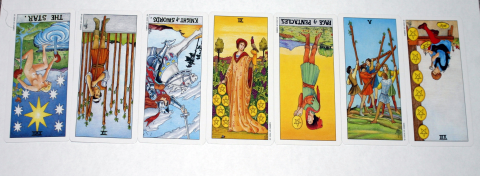
\includegraphics{image8-14-08.png}

\subsection*{The Reading}
The eight of swords shows a man with eight swords stuck in his back and
ear as he lies on the beach.  There is no blood coming from his body.
This image describes the ultimate in over reaction.  Where one sword
would've sufficed, eight have been used.  The lack of blood shows
surreality, as in the man may not actually be a man at all, as if eight
swords have been driven through a ghost, hallucination, or shadow of an
idea on this beach, right at the shore where the conscious meets the
subconscious.  I think that this card, as my `card of the day' of sorts,
is telling me to relax.  I have spent this time working with my
stressors --- getting away from some, integrating others --- and now I'm
creating more for myself by overreacting at imaginary things from the
depths of my subconscious.  With this in mind, I drew my reading for the
day, immediately surprised by only one upright card.

The Star, following immediately after The Tower, suggests a time of
healing.  Not only is the unconscious exposed and beginning to blend
with the conscious mind, but unlike The Tower, which describes the same
idea, The Star deals more with the calm after the storm --- the period
spent healing that rent caused by the fall from The Tower.  Reversed, we
are cut off from that calm, and that fear from our fall turns to
insecurity or even arrogance.  As it takes its place in my past
experience, I see that as an incomplete use of my flitting interests:
those things that distract me from stressors in order to help me heal
are not being carried out to completion, and instead of healing over,
I'm left with scars.  This echoes my desire to follow through with this
project to completion.  This, of all of my projects, is overt
self-therapy, as it's no secret that I am using this, in part, to help
get over a real ``Tower'' of a summer.

This moves into my expectations for this Work: the Nine of Wands shows a
man ready and wary, keeping his eyes out from enemies, ones that may or
may not still be enemies.  The card tells of wariness and strenght, but
also of seeing fights where there may in fact be none at all.  Reversed
twists that meaning to seeking a way out of this constant cycle, either
from being overwhelmed by the aversions or simply distressed by them.
While this is all well and good, it should be noted that sometimes these
defenses are built up for a reason, and should not be dropped lightly.
There are cases where such defenses are necessary, and I think I'm
focusing too much on these right now.  I think that opening myself up
through the cards is one case where I will \emph{have} to drop those
defenses and seek another way; I consciously know this, and expect
that this experiment will help.

The three cards of the Work group show what Pollack describes as
``\ldots{}situ-ations, influences, or attitudes that the person can use
or must overcome.''  In my case, more warnings are present.  The Knight
of Swords reversed suggests wildly casting about, showing a need to make
careful decisions and to be aware of my situation.  The Nine of
Pentacles is a card of success due to sacrifice; I need to be mindful
that this sacrifice really is for the better and not let the fact that I
am sacrificing something get in the way --- the reward is always greater
for the sacrifice.  Finally, the Page of Pentacles reversed warns again:
without a sense of hard work, all of the focus and grounded-ness of the
pentacles is liable to dissipate, leading to what Waite called
`prodigality'.

Taken together as a group these cards paint a picture of what needs to
be done.  While I know that I am working towards avoiding this casting
about ceaselessly for something with which to help myself, I will need
the Pentacles' focus and the sacrifice showin in the Nine.  To me, I see
this as sacrificing time and energy, both of which seem to be
increasingly parcelled out in today's world.  Free time is always seen
as valuable, and it's difficult to give some of mine up to a task that
requires such mental exertion and, honestly, leaves me intellectually
winded for a period afterwards.  I needn't be afraid of this sacrifice,
however, as expensing that energy will help me in at least two ways: not 
only with the therapy inherent in this project; but also as a sort of
exercise, building up my intellectual stamina, as it were, getting my
mind used to working in these intricate patterns.
%KnS R - wild casting about, requires careful decisions and awareness
%9P - success with sacrifice, if sacrifice seems too great, reconsider
%the value of the rewards we'll gain - always great
%PP R - without sense of hard work, dissipates; prodigality

Following the Work group of cards is the final combination of Outcome
and Result.  While Outcome stands for the likely way that things will
develop, Result implies a more personal side, showing how the outcome
with affect the subject or their reaction to it.  For my reading, these
cards came out fairly disheartening at first.  The Five of Wands
reversed suggests rules abandoned in this intellectual battle of mine, leading to
nastier combat.  I'll clearly have to do more to stick with this
interest, lest it fall by the wayside - perhaps things out of the
ordinary for me.  The Eight of Pentacles reversed on the other hand,
shows frustration and lack of fulfillment due to looking strictly for
success rather than working for the sake of work.  This meaning grated
on my nerves until I saw it as just another step in the path: not only
is success in the standard sense of strict completion unlikely, but I 
am almost certain to become frustrated by not really having an ending
point to this at all.  After all, this is only seventy-eight tarot
readings, which is only a little more than a fifth of a year if they are
done one a day!  I could change so much more, reading every day for the
rest of my life, and still never reach an end to this experiment, as
there is always more change to be had.  This is certainly something I
must learn to accept if I am to keep this project and others going
strong.
% 5W R - rules abandoned, battle is nastier, have to do more to
% stickwith interest?
% 8P R - frustration/unfulfilled from looking for Success, not work ?

\subsection{August 17, 2008}
\subsubsection*{The Background}
Last night, I drew another card to ponder for the next day or so and
picked the Nine of Swords from the Universal Waite deck\cite{tarotRWS}.
This card contains a distressing image of someone buried deep in
emotional agony, sitting up in bed while nine swords hang in the air
above and behind them.  While the card usually stands for that
withdrawal into self that comes with tsuch emotional pain, it can also
represent, particularly while reversed or ill-dignified, oppression.  In
fact, Rachel Pollack specifically mentions sexuality as the reason for
the oppression, and that brought to mind work.

At my day job, working as technical support in the campus library, my
direct supervisor quit late last year and was replaced with someone
twice as competent as he was.  My old supervisor was very good at
keeping the library up and running, and my new supervisor is better,
going further by doing things to make the library work even more
smoothly.  However, while my old supervisor acted fairly immature and
made crude jokes ceaselessly, my new supervisor far outstrips him in
this category, with every word and action showing the twelve-year-old
that he still thinks he is.

While I don't believe that he is actively oppressing me because of my
sexuality --- I doubt he even knows, and they are pretty clearly jokes,
my Indonesian coworker gets his fair share of terrorist jokes --- it
does lead to a decidedly uncomfortable environment to be working in at
times.  Perhaps I'm just a sensitive person, but I would enjoy not
having this stigma hanging over my workplace.  How can I work more
effectively with this?  Is coming out to my boss the right thing, or
should I follow my own suggestion and not let my sexuality interfere
with my job, since the former has no place in the latter?

\subsubsection*{The Drawing}
Still using the Universal Waite deck, I decided to make up a spread on
the spot.  The layout would consist of two piles related to two `header'
cards.  One header card would stand for what I saw in my boss and the
other would stand for a different view-point on the situation: that of 
my boss.  I would draw two cards at a time, one for each pile,
and read the two cards in a general matter to gain perspective on the
situation, drawing until I feel that I've got a better idea of what's
going on.

\begin{itemize}
  \item Theme for the reading: Nine of Swords
  \item My header card: Knight of Cups.
  \begin{enumerate}
    \item Four of Pentacles
    \item Five of Wands
    \item The Devil
    \item Six of Wands
  \end{enumerate}
  \item The other header card: Knight of Wands.
  \begin{enumerate}
    \item King of Wands
    \item Four of Swords
    \item Death
    \item Eight of Swords
  \end{enumerate}
  \item Final card: Ace of Wands
\end{itemize}
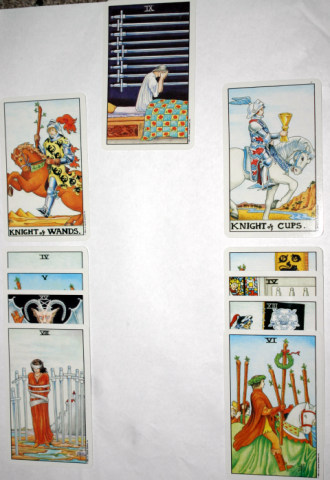
\includegraphics{image8-17-08.png}

\subsection*{The Reading}
I initially selected the header card for my boss, since his attitude at
work recently has reminded me of little else, what with the way the
Knight of Wands rushes into battle, usually without any sort of plan.
Recently, my boss has been fixing things `shotgun style' at work, just
replacing parts and hoping they're the right ones, and that replacing
them will fix the issue.  I chose my own header card in much the same
way, with the Knight of Cups' more reticent nature, particularly as
applied to how I feel about dealing with my boss.  It wasn't until I got
halfway through the spread that I noticed that they were elementally
ill-disposed towards one another.

Looking at my boss's header card, the first thing I notice in the picture
itself is the flashiness of the uniform.  My boss doesn't dress flashy,
but he does act in such a way as to draw attention to himself, and I
find this particularly apt.  In my own card, I first noticed that the
Knight doesn't look at anything other than the cup, keeping his fist
wrapped tightly around his horse's reigns, even though it looks as if
the horse would really rather like a drink of that stream in front of
him.  For myself, I see this as me focusing a little too hard on this
issue, perhaps at the expense of those issues around me.  The rest of
the reading proceeded more as a dialog.

I drew the first two cards at once and laid them beneath the two header
cards: the Four of Pentacles and the King of Wands.  The traditional
meaning of the King was not, as I found, very applicable.  Instead, the
card, as being a vertical transmutation of my boss's Knight, very
plainly spoke of my desires for my boss to grow up.  His homophobic
jokes are so\ldots high-school.  Not only am I in college, but he is
nearing thirty, and it's well past time for him to get on with work and
out of this party stage.  His card, on the other hand, spoke of
defenses.  The miser in the Four of Pentacles protects his heart and
mind with defensive layers, and even his feet are covered to, perhaps
inadvertently, block that symbolic connection with the earth and thus
everyone else.  This card responded to the King by saying, ``I use that
humor to cover up and hide problems deeper than this.''

The second two cards were drawn.  My Four of Swords suggests relaxation,
retreating from the while, taking things in stock.  I believe that this
is me telling my boss to relax, calm down, maybe step back and take in
the world from a different point of view rather than rushing forward.
Perhaps then he would be easier to reason with, rather than attempting
to talk with that joker of a mask he wears.  In response, his Five of
Wands suggested that there is no real reason to do such a thing.  ``Life
is just a game,'' it said.  ``So long as we follow the rules and do our
jobs, it doesn't matter.''

My exasperation was brought forth in the the next two cards, both Major
Arcana.  Death, for my card, begged for change and transition.  ``The
game needs to change --- you need to change --- so that we can both do
our jobs more effectively''  My boss's card, the Devil, shrugs that off
with comfort and complacency.  ``This may not be my true self, and may
just be a mask, but there's no reason to change; you know and I know
that neither of us are too enthused about our jobs and they're hardly
challenging either of us.  Office humor helps keep things sane for both
of us, and you know that.''

At this point in the reading, I felt like I had a better grasp on the
situation.  I know my boss really is just joking: whether he is
homophobic or not doesn't enter into it much at all, I think --- this is
just a way to keep himself sane at work.  However, it is affecting the
way I feel about my job and the way I perform at work, to a small
extent.  Rather than joining in conversations at work as I used to, I'm
more inclined to just sit and listen, unwilling to participate in the
things I disagree with.  

The social activist Unitarian in me would like
to tell my boss how inappropriate that is in any setting; while I'm
hardly `tough', there are those that aren't as thick-skinned as I am
when it comes to this sort of thing, and he should avoid being hurtful
towards anyone.  Still, I'm wary of opening up in this situation lest it
make things strained between my boss and myself, or, worse, that he'll
get in trouble with someone higher up than him --- as I mentioned
before, he really turned the workplace around, productivity-wise.
Curious and willing to try, I drew two more cards with the intent of
seeing how this dynamic may extend into the future.

The Eight of Swords shows a woman actively oppressed, bound and
blindfolded and surrounded by swords.  However, her oppressors are
nowhere in sight and the swords only block her on one side.  This is an
oppression that she has come to expect, whether out of cynicism or
weakness.  If I were to accept my oppression like this card suggests
being under my heading, then my boss's card, the Six of Swords, may be
in his future: Victory.  The man rides crowned on his horse, riding in a
victory parade, completely unharmed.  He has done nothing and he has
won and I have lost, dignity trampled.

Frustrated, I drew one final card, just to look for something more
optimistic.  The Ace of Wands is just what I needed.  The embodiment of
the energy of the Wands, happiness and joy as a gift from that inner
strength I know we all have.  I know what I have to do.

I will have to confront my boss on this matter soon.

\subsection{August 18, 2008}
\subsubsection*{The Background}
I feel oddly blank.  Distressingly so.

\subsubsection*{The Drawing}
Exploring the void with the Universal Waite\cite{tarotRWS}.

\begin{enumerate}
  \item Four of Pentacles.
  \item Death
  \item Seven of Pentacles
  \item Eight of Pentacles
  \item Judgement
  \item Two of Pentacles
  \item The High Priestess
  \item The Star
  \item Nine of Pentacles
  \item Eight of Swords
\end{enumerate}
\emph{[No Image]}
%\includegraphics{file}

\subsection*{The Reading}
I'm unhappy about feeling as blank as I am.  I drew cards aimlessly and
interpretted them as they came, letting the meanings come rather than
resorting to a book or even caring about what I consciously knew about
the cards.  No reversals or anything were used.  Just one card at a
time.

\subsubsection*{The First Card}
The Four of Pentacles strikes me as a smug card.  I know that it should
be seen as smug on the outside and hurt on the inside, but sometimes,
it's so hard to get past the little twist of the man's eyebrows, that
little bit of contentment.  Or the way he holds the Pentacle on his lap,
deliberately casual, with his chin resting on his hand and the other arm
in his lap, as if he wants you to notice it.  A man hiding behind his
money.

\subsubsection*{The Second Card}
Death, more than any other card, reminds me of the passage of time.
Nothing can stop that horse.  The king couldn't stop it, nor will the
cleric, the woman, nor the child.  The sun still shines, the river still
flows with the boat on it.  Death is inevitability.

\subsubsection*{The Third Card}
The Seven of Pentacles is a card of hard-earned rewards, but now I'm
noticing the slightly unhappy cast to the farmer's face, as if it wasn't
quite as much as he was expecting this year, or if the rewards aren't
quite up to his high standards.  It is working towards perfection but
never quite getting there - doing great things but driving yourself
always harder.

\subsubsection*{The Fourth Card}
In the Eight of Pentacles, I see a person doing what they love, having
retreated from society or societal norms to do so.  It is caring more
about your art than those who might appreciate it, and doing so because
it is your job, as ordained by the person you are, rather than any
authority.  Some people work at what they do because that is what they
must do.

\subsubsection*{The Fifth Card}
Judgement shows all those nameless, faceless people who follow an idea.
They are sheep, and happier for it.  It is hard to see this card as bad,
though, as one should never underestimate the power of people in groups
following an idea.  Still, it makes me feel like an outsider.

\subsubsection*{The Sixth Card}
The Two of Pentacles seems almost to be a hallucination at this point.
It is the view of work being done by an outsider who doesn't know what
is going on.  It is a verb, describing the action of an act so esoteric
it seems to be magic.  Even the ships seem perplexed.

\subsubsection*{The Seventh Card}
The High Priestess is guarding something, but you'll never get to know
what.  Her face is so composed, so blank and she's so still that not
even her expression or body language can give away the landscape behind
her, however breathtaking it might be.  She still holds the law in her
hand, so I'm afraid to ask sometimes.

\subsubsection*{The Eighth Card}
The Star works behind the scenes doing what must be done, even when
things fall apart.  It is the inner workings of the emotional mind that
keeps me going even when I'm crashing.  She is the inner alchemist that
churns and toils to keep the juices flowing, as it were, to keep the
bellows moving and the fire stoked in my mind and heart.

\subsubsection*{The Ninth Card}
The Nine of Pentacles is distraction.  Someone did the work and it's
there to appreciate, but only in a vague sense of the word, strolling
through the gardens and taking it in, while really you're thinking about
who did what with whom last week, or something to appreciate in a
picture in the office.  And the bird who may recognize any sort of
beauty has a hood on, kept from seeing what's really around for the
whims of another.

\subsubsection*{The Tenth Card}
The Eight of Swords is martyrdom, being bound to the stake of sorts.  It
is willingly giving yourself up to those hostile forces around you.  Or,
and I hate to think about it, it is being too weak and caving in to
those whims.  Doing what you're told because you haven't the strength to
do what you must.

\subsubsection*{Analysis - after the fact}
I had to wait until the next day to finish analyzing the cards ---
usually, I outline everything and take a day or two to add in the
details --- as soon as I drew the last card, the blankness of emotion,
of intellect, and of Self drove me to bed, leaving me to be enveloped
somewhere more comfortable than in front of my computer.  As I'm feeling
much different today, I shall try to finish this chapter.  My aim is to
recall last night as best as I can and provide an interpretation based
on what I wrote, and then go back through the cards and provide a new
interpretation using more traditional definitions.

The ten cards I drew and interpretted briefly last night outline a path.
Briefly, smug and content in my comfortable new major with my knowledge
and ease of composing, shown in the first card, changes little in the
second card.  No one cares at work, my music still isn't getting
performed, and I feel no closer to graduating.  The third card is partly
my realization of this and partly that part of me that wishes to excel,
needing to work harder; and the fourth card shows me about where I am
now: feeling the need to retreat a little in order to do what I like
doing, since it sometimes feels as if I've chosen a major that no one
sees the use of, least of all my parents.

The next several cards seem much more speculative.  Begining with the
Fifth card, the music world of today, particularly in education and
popular circles is shown as sheep following a leader, some composer (the
sixth card) working their magic and becoming successful by writing the
music that sells with good marketing rather than good musicianship.  The
seventh and eighth cards are likely what I would do when confronted with
such an individual.  While I work my own `magic' with my music, I seem
more to be incomprehensible, but, running my own publishing business, I
hold the law in my hands.  The eight card shows, in particular, my
realiziation of this, of trying to keep alive a portion of my art that
no longer serves the function of art, without an audience.  

The ninth card shows more of the world around me, of music and art in
general falling by the wayside, as it has in the past few years, to
background noise.  Music that one hears in restaurants and on the radio
just because it's there, not for the purposes of enjoyment or
enlightenment.  The tenth card is my big ``I told you so'' moment to the
world.  I left the education system to get away from the way this
country seems to embrace that background-noise ideal.  I tried to change
that with my publishing company and all I did was cause trouble.  Take
that.  Or else the second meaning comes into play and I wind up hurting
for money, writing that very music that I despise so much.

Reading strictly from the rather stupid subconscious seemed to be easier when pulling
definitions, but stringing together the meanings into a coherent
analysis was certainly much more difficult.  When I apply the conscious
intellect inherent in analysis of the cards, though, the meaning becomes
much more evident and easier to string together into a time-line without
having to stretch so much.  This proves my earlier thoughts, that tarot
requires all levels of consciousness in order to be used successfully.
As such, many of the meanings I pulled from inside are still accurate in
a way: the overall premise of the storyline changes, but the problem
remains the same, as that of the weakening world of art.

Whereas I mentioned I was smug and content in my musicianship, a more
traditional standpoint shows less about the musicianship than about the
musician.  I'm creating structure in this world through my art, but also
using it to turn inwards and as a protective shell for myself, in the
first card.  The second card traditionally means changed, and I chose
the meaning of inevitability.   The two go hand in hand, and perhaps
this is a signal of change to come, what with my growing business.
Perhaps my structures should be more productive than they are now.  The
original meaning of the third card is indeed a much happier one than
I've chosen, but along the same lines of completion.  I think that mine
still applies, however, the constant need to excel is not a bad need to
have --- the work is not yet done, and this is shown in the next card.
The work is never done.

Here the reading diverges much more from what I saw in the subconscious
drawings.  The fifth card shows a call to change from within (or,
rather, a call to recognize what change has already happened), and the
sixth card represents the balancing act that is life in general.  Rather
than the outside perspective I saw before, these two cards indicate a
rebalancing of my life.  While composition will still be very important
to me, I think I need to realize that I've found my calling in life more
in the publishing of great new works of music.  

The High Priestess represents passivity, possibly in excess.  I do still
believe that music and art are not currently being herded to a very
constructive destination by both artists and policy makers in this
country, but I think that now is a good time to work against that with
my own music and my company to help get the music of others out there in
the open.  If I hesitate too long, my work will be ineffectual against
this slow drift into mediocrity.  The Star as the eigth card, however,
does caution a pause to build my resources, to grow into this position
without rushing headlong into it.  The Star and The Tower often suggest
each other, and I see The Tower looming on either side of this card:
either from rushing the process or waiting too long, I'm liable to
destroy myself.

The final two cards show offer a bit of advice about the way things are
running.  First of all, the Nine of Pentacles as the ninth card suggests
the recognition of rewards.  This has multiple meanings in context --- I
must recongize the greatness of the composers who ask to publish through
my company, I must recognize the need for my company, and I must
recognize the importance of my customers, for they are literally my
financial reward.  However, I must be careful of oppression, as shown by
the final card.  I should avoid blindfolding myself and oppressing
myself by painting myself into a corner, as it were, and I must also
avoid adding that blindfold to others, both composers and customers.
Those other styles of music do have a place in our world, and I've been
good so far about sending artists interested in that to other venues
more willing to publish their works, but I will need to keep up with
that so that I don't discourage them.  I will also need to keep an open
mind about what I will be able to publish, lest I deprive the world of
that music, or the composers of their recognition.

These two readings were particularly helpful to me.  I learned the place
of each of the levels of consciousness in the Tarot workspace, as well
as my limitations in reading from the spot.  I hope that my skills as a
reader will improve through this experiment, and I also hope that what I
learn from my readings will remain applicable in my business throughout
my life, as this reading seems to have proved to me just how important
this idea is.  As a pertinent final note, my card for the day was the
Seven of Swords, cautioning leaping into things without a plan.  This
applies to both the business as discussed above, but also my method of
reading.  I did enjoy the looseness without a spread, but I should plan
to work harder on reading on all levels.



%%%%%
\section{Analysis}
The analysis of this experiment will be written when all data is
collected, in order to more properly answer the questions posed.
%answer questions with experimental data

\bibliographystyle{apalike}
\bibliography{biblio}
\end{document}
